% =========================================================
% CHAPTER 14: RESULTS AND SCREENSHOTS
% =========================================================
\chapter{Results and Visual Evidence}
\label{chap:results}

\section{Machine Learning Experimental Results}
The machine learning component was rigorously evaluated on the PaySim financial transaction dataset using stratified holdout evaluation ($254,505$ test instances) and 5-fold cross-validation.

\subsection{Holdout Confusion Matrices}
Figures~\ref{fig:cm_rf_tuned}, \ref{fig:cm_xgb_tuned}, \ref{fig:cm_dt}, and \ref{fig:cm_lr} present the empirical confusion matrices generated across the candidate models during evaluation.

\begin{figure}[htbp]
    \centering
    \begin{subfigure}[b]{0.48\textwidth}
        \centering
        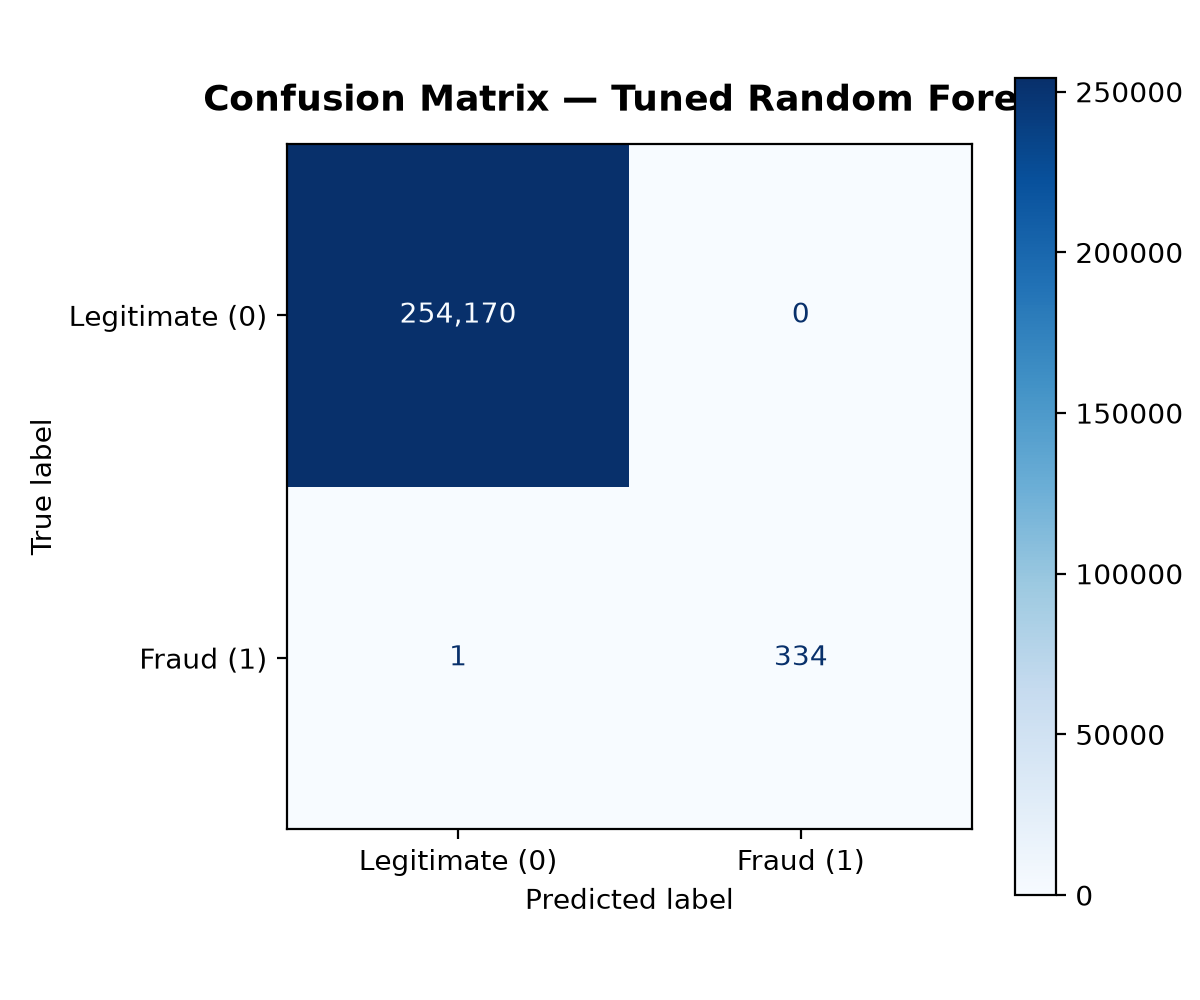
\includegraphics[width=\textwidth]{figures/random_forest_tuned_confusion_matrix.png}
        \caption{Tuned Random Forest (Selected Production Model: 0 False Positives, 334 True Positives)}
        \label{fig:cm_rf_tuned}
    \end{subfigure}
    \hfill
    \begin{subfigure}[b]{0.48\textwidth}
        \centering
        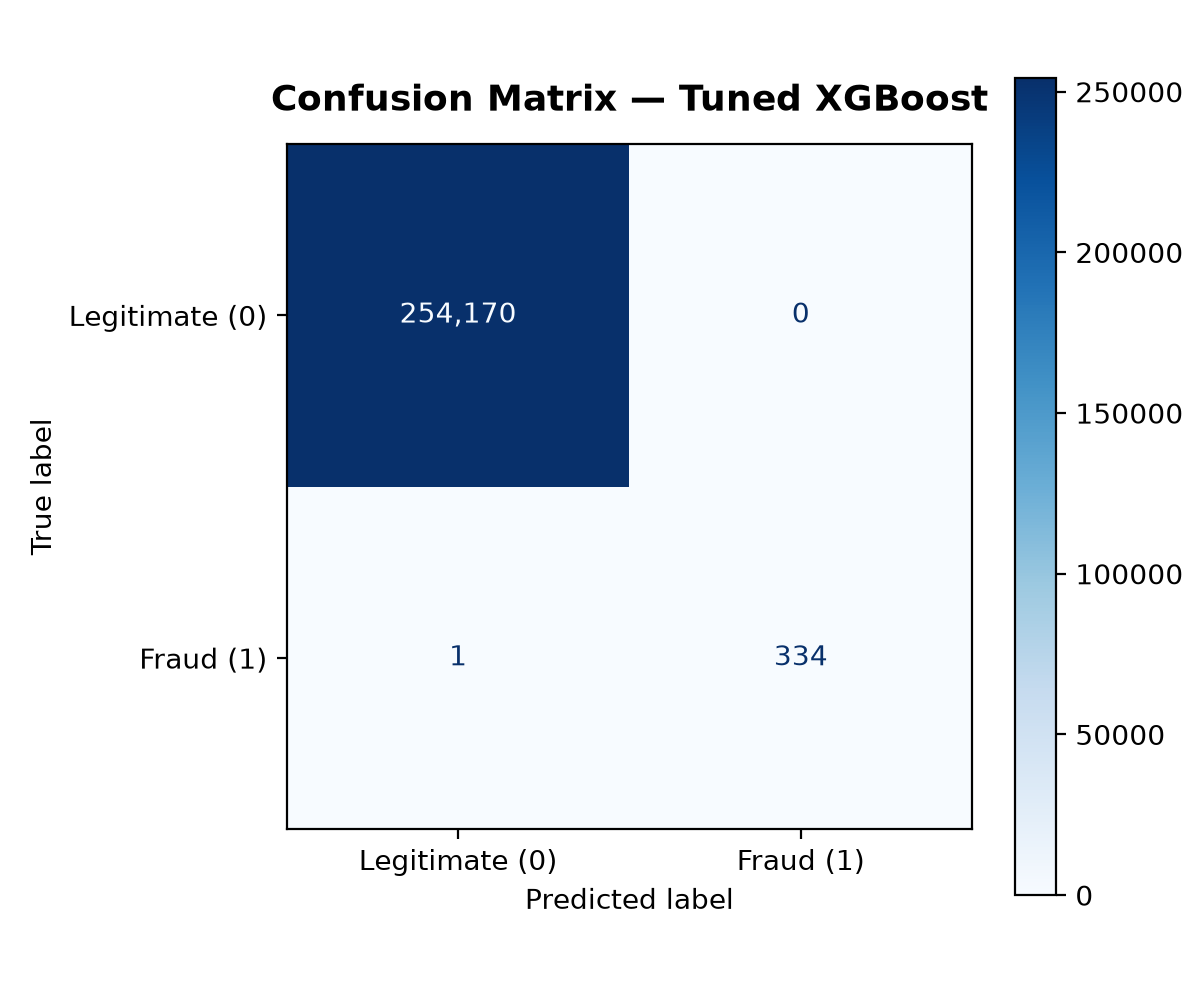
\includegraphics[width=\textwidth]{figures/xgboost_tuned_confusion_matrix.png}
        \caption{Tuned XGBoost Benchmark (0 False Positives, 334 True Positives)}
        \label{fig:cm_xgb_tuned}
    \end{subfigure}
    \vspace{0.4cm}
    \begin{subfigure}[b]{0.48\textwidth}
        \centering
        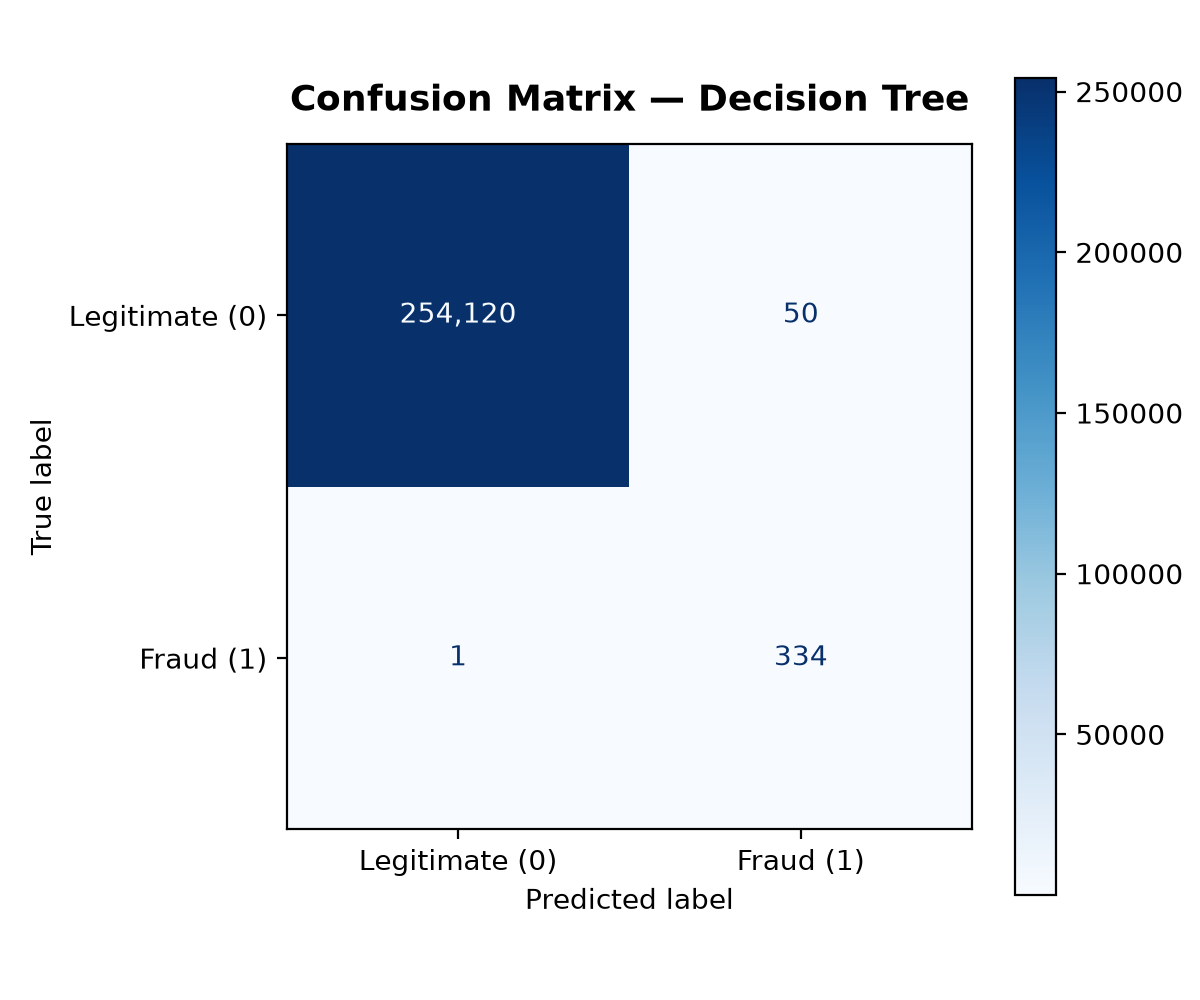
\includegraphics[width=\textwidth]{figures/decision_tree_confusion_matrix.png}
        \caption{Decision Tree Baseline (52 False Positives)}
        \label{fig:cm_dt}
    \end{subfigure}
    \hfill
    \begin{subfigure}[b]{0.48\textwidth}
        \centering
        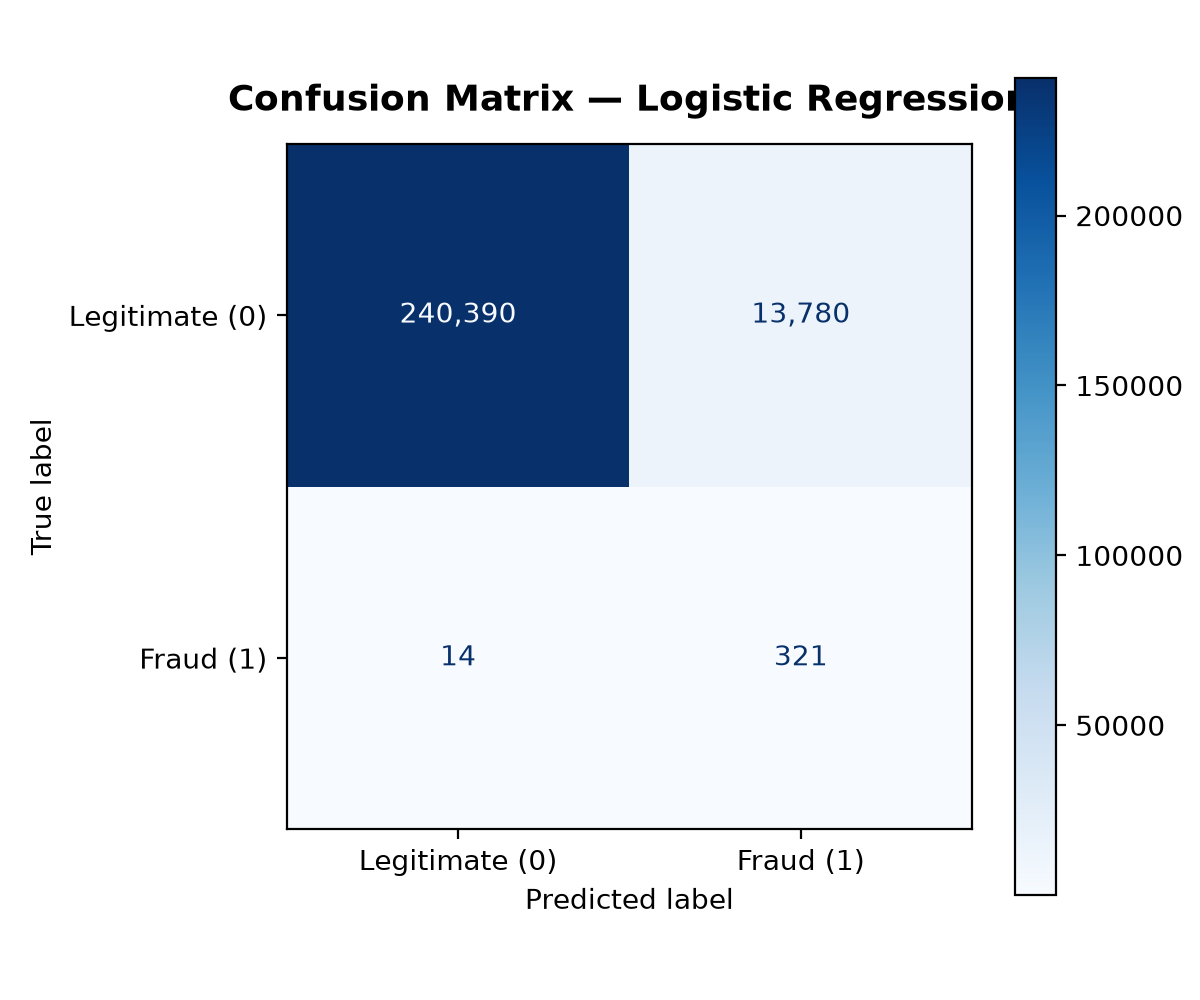
\includegraphics[width=\textwidth]{figures/logistic_regression_confusion_matrix.png}
        \caption{Logistic Regression Baseline (13,780 False Positives)}
        \label{fig:cm_lr}
    \end{subfigure}
    \caption{Empirical Confusion Matrices across Evaluated Machine Learning Models}
    \label{fig:all_confusion_matrices}
\end{figure}

\subsection{Model Comparison Benchmark Chart}
Figure~\ref{fig:model_comparison_chart} illustrates the performance comparison across Precision, Recall, F1-Score, and PR-AUC.

\begin{figure}[htbp]
    \centering
    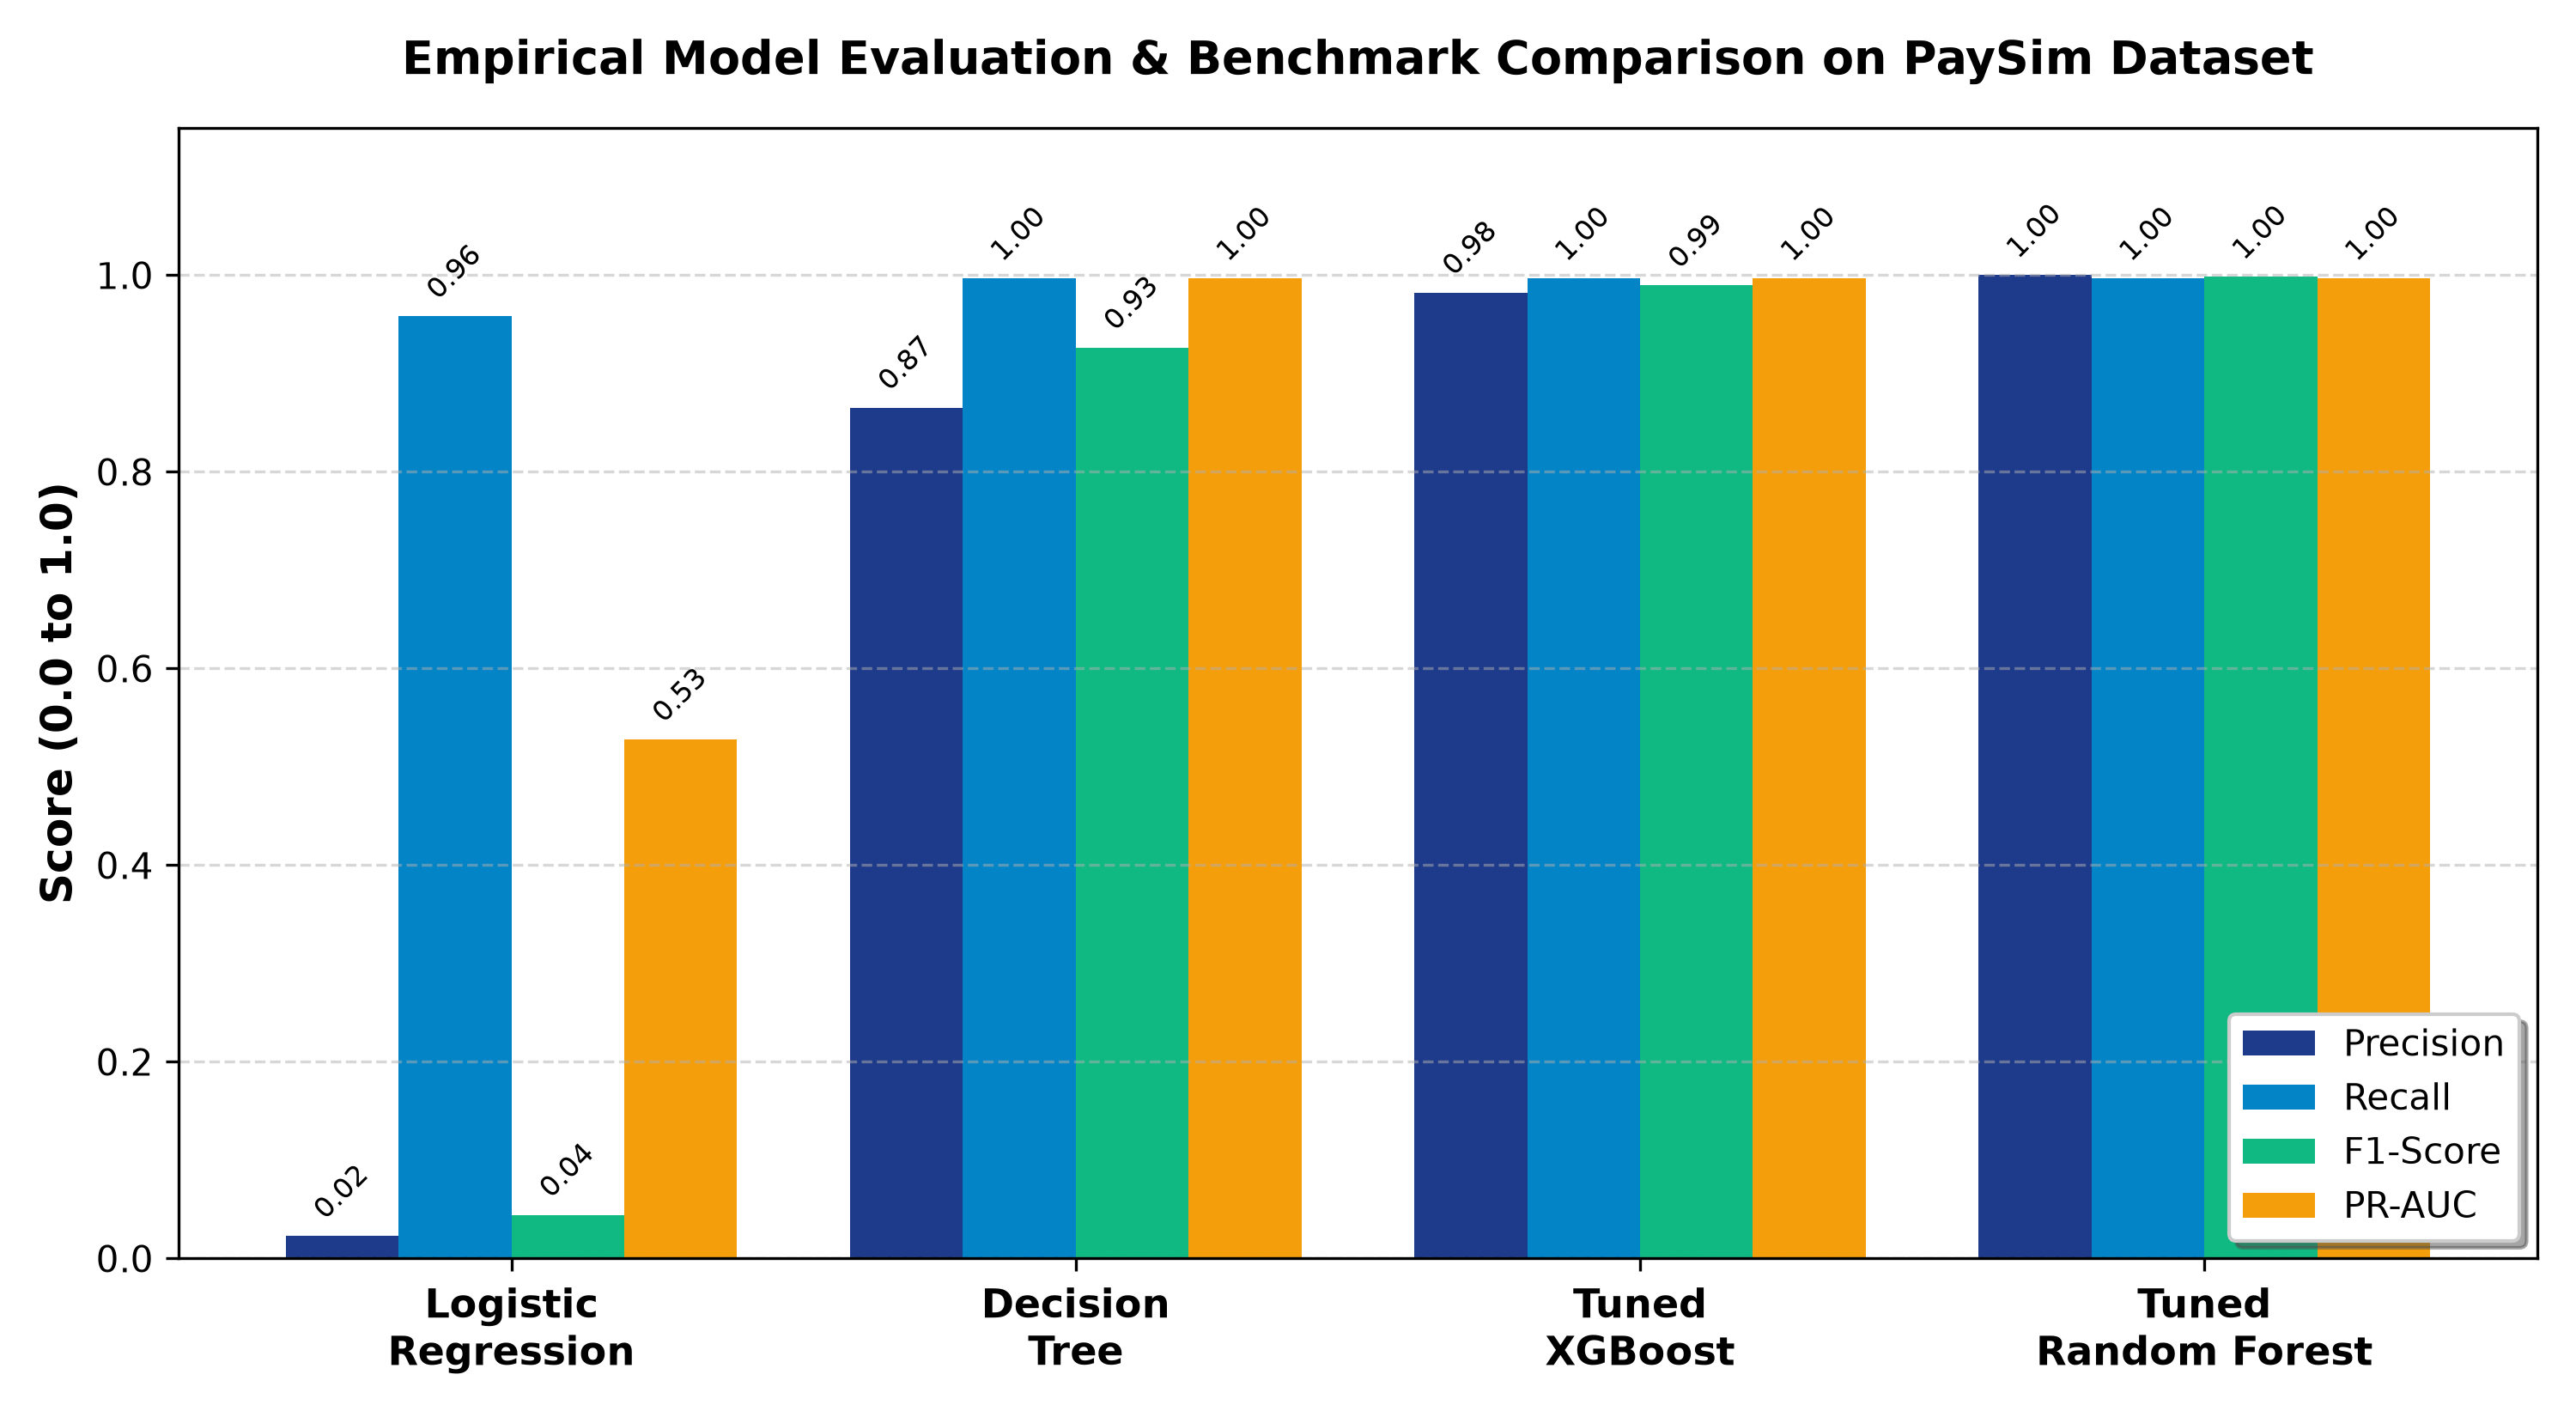
\includegraphics[width=0.92\textwidth]{figures/model_comparison_chart.png}
    \caption{Model Comparison Benchmark across Key Precision, Recall, F1, and PR-AUC Metrics}
    \label{fig:model_comparison_chart}
\end{figure}

\subsection{Feature Importance and SHAP Attributions}
Figure~\ref{fig:feature_importance_chart} displays the top 10 most influential features determined through mean absolute SHAP attributions.

\begin{figure}[htbp]
    \centering
    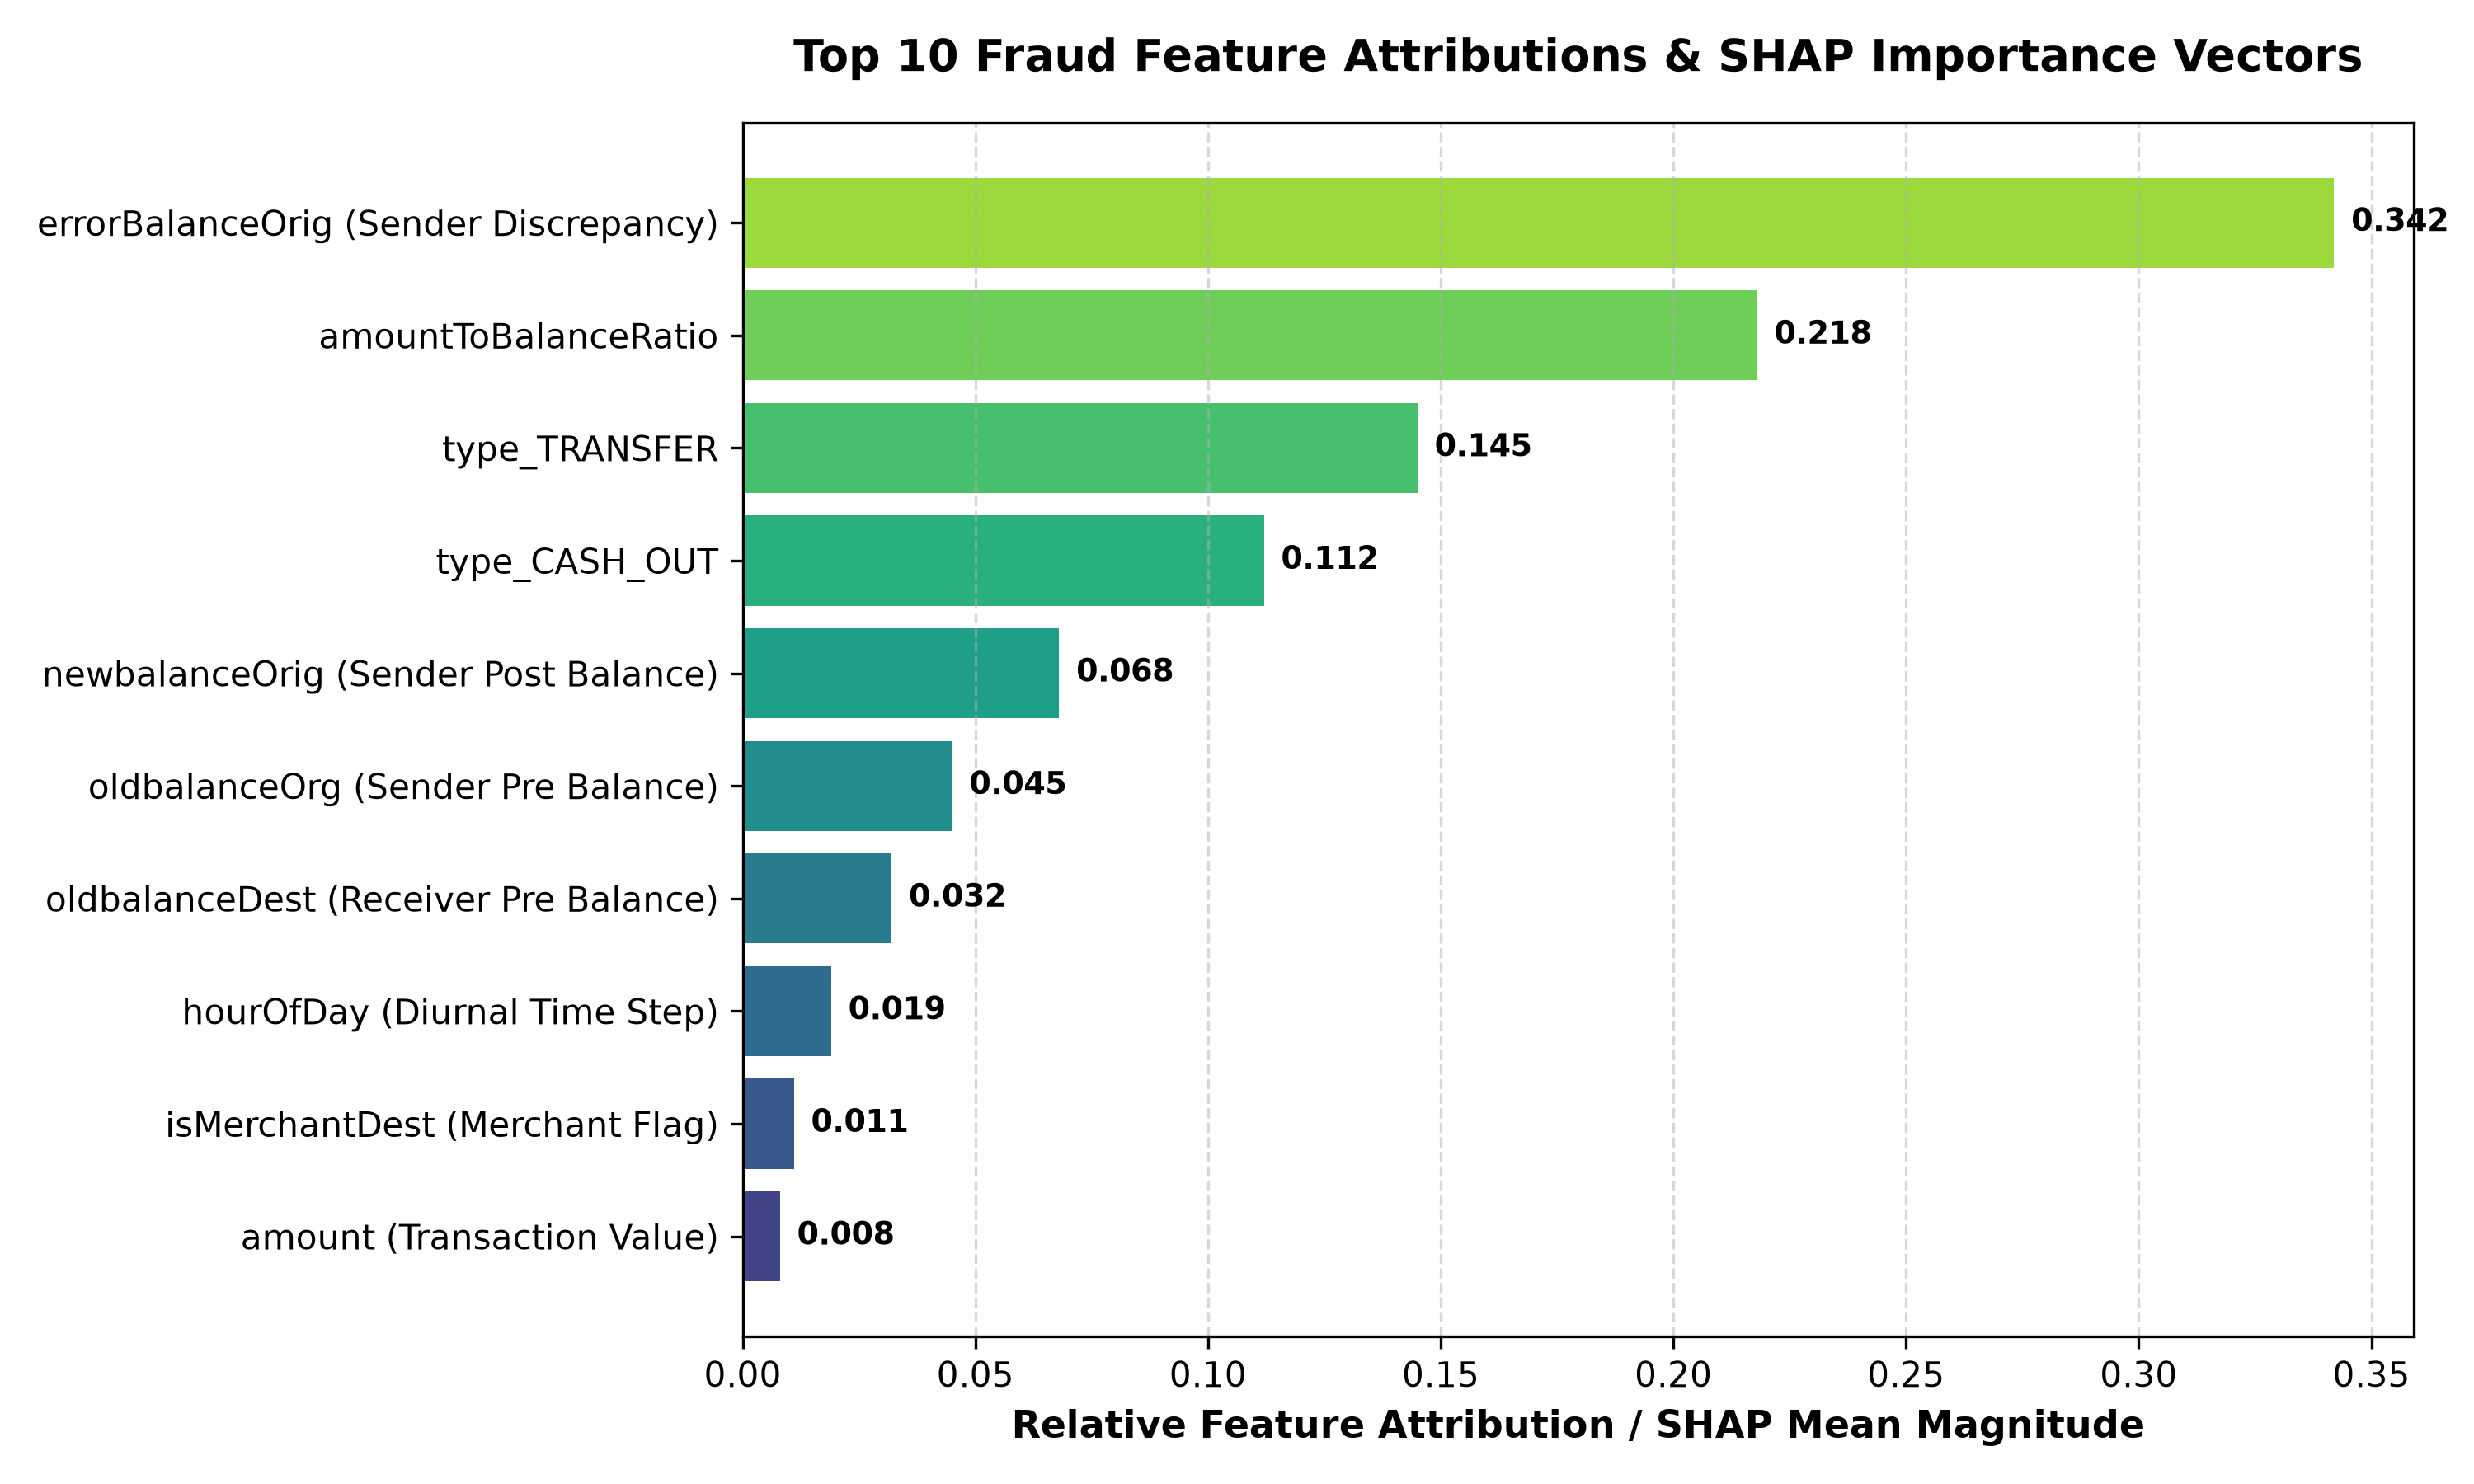
\includegraphics[width=0.92\textwidth]{figures/feature_importance_chart.png}
    \caption{Top 10 Feature Importance Vectors and Mean SHAP Values}
    \label{fig:feature_importance_chart}
\end{figure}

\section{System Interface and Operational Views}

\subsection{Customer Portal Views}
\begin{enumerate}[label=\arabic*.]
    \item \textbf{Customer Dashboard}: Displays real-time account balances, Virtual Payment Address (VPA), quick-action transfer buttons, and recent transaction history cards.
    \item \textbf{Payment Simulator Interface}: Allows customers to select transfer mechanisms (VPA, Phone, QR Code), enter recipient details, input amounts, and authorize transactions using their 4-digit PIN.
    \item \textbf{Real-Time Risk Assessment Modal}: Immediately displays the calculated risk score ($0-100$) and visual status tag upon transaction submission.
    \item \textbf{Step-Up Email OTP Challenge Modal}: Renders an interactive 6-box numeric OTP entry form with an active 180-second countdown timer.
    \item \textbf{SHAP ``Why Was This Flagged?'' Drawer}: An interactive off-canvas drawer that presents horizontal green/red feature attribution bars and plain-English explanatory text.
\end{enumerate}

\subsection{Security Operations Center (SOC) Views}
\begin{enumerate}[label=\arabic*.]
    \item \textbf{SOC Incident Triage Table}: Displays open high-risk and critical-risk alerts with severity badges, timestamps, and customer email addresses.
    \item \textbf{SOC Telemetry Dashboard}: Features dynamic Chart.js charts showing hourly transaction volumes, risk score distributions, and fraud rates.
    \item \textbf{Case Investigation Modal}: Displays full SHAP technical attributions ($E[f(x)]$ vs $f(x)$) and allows security analysts to submit resolution notes.
\end{enumerate}
